\begin{figure}[ht]
\centering
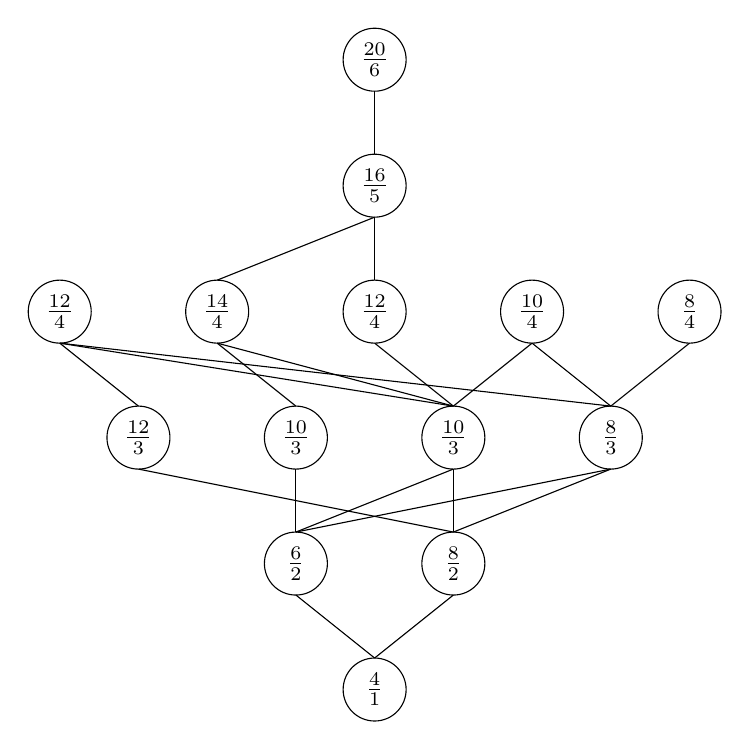
\begin{tikzpicture}
  [scale=.04,auto=left]
  
  \def\X{40}
  \def\Y{0}
  
  \def\x{\X -10}
  \def\y{\Y}
  
  \draw  (\x +10,\y +5) circle [radius=10cm] node {$\frac{4}{1}$};

  \def\x{\X -35}
  \def\y{\Y +40}
    
  \draw  (\x +10,\y +5) circle [radius=10cm] node {$\frac{6}{2}$};
  
  \draw  (\x +10,\y -5) -- (\x +35,\y -25);
  
  \def\x{\X +15}
  \def\y{\Y +40}
    
  \draw  (\x +10,\y +5) circle [radius=10cm] node {$\frac{8}{2}$};
  
  \draw  (\x +10,\y -5) -- (\x -15,\y -25);
  
  \def\x{\X -85}
  \def\y{\Y +80}
    
  \draw  (\x +10,\y +5) circle [radius=10cm] node {$\frac{12}{3}$};
  
  \draw  (\x +10,\y -5) -- (\x +110,\y -25);
  
  \def\x{\X -35}
  \def\y{\Y +80}
    
  \draw  (\x +10,\y +5) circle [radius=10cm] node {$\frac{10}{3}$};
  
  \draw  (\x +10,\y -5) -- (\x +10,\y -25);
  
  \def\x{\X +15}
  \def\y{\Y +80}
    
  \draw  (\x +10,\y +5) circle [radius=10cm] node {$\frac{10}{3}$};
  
  \draw  (\x +10,\y -5) -- (\x +10,\y -25);
  \draw  (\x +10,\y -5) -- (\x -40,\y -25);
  
  \def\x{\X +65}
  \def\y{\Y +80}
    
  \draw  (\x +10,\y +5) circle [radius=10cm] node {$\frac{8}{3}$};
  
  \draw  (\x +10,\y -5) -- (\x -40,\y -25);
  \draw  (\x +10,\y -5) -- (\x -90,\y -25);
  
  \def\x{\X -110}
  \def\y{\Y +120}
    
  \draw  (\x +10,\y +5) circle [radius=10cm] node {$\frac{12}{4}$};
  
  \draw  (\x +10,\y -5) -- (\x +35,\y -25);
  \draw  (\x +10,\y -5) -- (\x +135,\y -25);
  \draw  (\x +10,\y -5) -- (\x +185,\y -25);
  
  \def\x{\X -60}
  \def\y{\Y +120}
    
  \draw  (\x +10,\y +5) circle [radius=10cm] node {$\frac{14}{4}$};
  
  \draw  (\x +10,\y -5) -- (\x +35,\y -25);
  \draw  (\x +10,\y -5) -- (\x +85,\y -25);
  
  \def\x{\X -10}
  \def\y{\Y +120}
    
  \draw  (\x +10,\y +5) circle [radius=10cm] node {$\frac{12}{4}$};
  
  \draw  (\x +10,\y -5) -- (\x +35,\y -25);
  
  \def\x{\X +40}
  \def\y{\Y +120}
    
  \draw  (\x +10,\y +5) circle [radius=10cm] node {$\frac{10}{4}$};
  
  \draw  (\x +10,\y -5) -- (\x +35,\y -25);
  \draw  (\x +10,\y -5) -- (\x -15,\y -25);
  
  \def\x{\X +90}
  \def\y{\Y +120}
    
  \draw  (\x +10,\y +5) circle [radius=10cm] node {$\frac{8}{4}$};
  
  \draw  (\x +10,\y -5) -- (\x -15,\y -25);
  
  \def\x{\X -10}
  \def\y{\Y +160}
    
  \draw  (\x +10,\y +5) circle [radius=10cm] node {$\frac{16}{5}$};
  
  \draw  (\x +10,\y -5) -- (\x +10,\y -25);
  \draw  (\x +10,\y -5) -- (\x -40,\y -25);
  
  \def\x{\X -10}
  \def\y{\Y +200}
    
  \draw  (\x +10,\y +5) circle [radius=10cm] node {$\frac{20}{6}$};
  
  \draw  (\x +10,\y -5) -- (\x +10,\y -25);
\end{tikzpicture}
  \caption{The numbers \(h(G)\) for all cut-minimal graphs on 6 vertices}
  \label{figure2:Figure 2}
\end{figure}
